\documentclass[11pt, fancy, bibstyle=apalike, cite=authoryear]{elegantbook}


%%%%%%%%%%%%%%%%%%%%%%%%%
%				Packages

\usepackage[ruled,vlined]{algorithm2e}

%\usepackage[style=authoryear,
%	bibstyle=authoryear,
%	citestyle=authoryear,
%	natbib=true,
%	hyperref=true,
%	backref=true,
%	abbreviate=true]{biblatex}
%	\addbibresource{master_references.bib}

\usepackage{wrapfig}

\usepackage{hyperref}
\hypersetup{
	colorlinks=true,
	linkcolor=cyan,
	filecolor=magenta,
	urlcolor=cyan,
	citecolor=green
}


\usepackage{pythonhighlight}
%	Python snippit
%		\begin{python}
%			def f(x):
%			return x
%		\end{python}
%	inline Python
%		\pyth{ <code>  }
%	load external Python file from line 23 to line 50
%		\inputpython{python_file.py}{23}{50}

%%%%%%%%%%%%%%%%%%%%%%%%%
% 				Custom environments
% \newenvironment{<env-name>}[<n-args>][<default>]{<begin-code>}{<end-code>}
\newenvironment{quest}{\begin{enumerate}[label=\bfseries Q: ]\bfseries}
	{\end{enumerate}}
\newenvironment{ans}{\par\normalfont}{}

\def\cloze{\textbf{(cloze) }}

%%%%%%%%%%%%%%%%%%%%%%%%%
% Title Details
\title{Daily Notes}
\subtitle{2020 \LaTeX{} doc}
\author{Unique Divine}
\institute{Elegant\LaTeX{} Program}
\date{April 12, 2020}
%\version{3.11}
\bioinfo{Bio}{Information}
\extrainfo{Victory won\rq t come to us unless we go to it. }
\logo{logo-blue.png}
\cover{cover.jpg}



%%%%%%%%%
\begin{document}
%%%%%%%%%

\maketitle
\frontmatter
\tableofcontents

%-------
% Body
%-------
\mainmatter

\chapter{Introduction}

\section{A Commonplace (Book)\footnote{\href{https://en.wikipedia.org/wiki/Commonplace_book}{Wikipedia : Commonplace Book}}}

A commonplace book is a system for writing down and sorting all manner of tidbits: quotes, anecdotes, observations, and information gleaned from books, conversations, movies, song lyrics, social posts, podcasts, life experiences, or anything else that you might want to return to later.

It's called a commonplace it's an aggregate, an all-encompassing system for storing all of the the most important points you learn in  one common place—a central resource that makes it easy to find, re-read, and utilize each piece of wisdom you have obtained.


\footnote{\href{https://www.masterclass.com/articles/how-to-keep-a-commonplace-book\#who-uses-commonplacing}{``What Is a Commonplace Book?'' (Article)} }



\section*{Why? | The Purpose of this Commonplace Book}

\subsection{We are at war.}

Constantly seeking out new experiences and opportunities to grow. We employ active recall methods, watch videos, lectures, and seminars. We listen to mentors and podcasts, captivated by the new insights and perspectives that enter our psychology.

As voracious learners, we are in a forever war

\subsection{Save Hours on Research}

\subsection{Find Unexpected Connections}

\subsection{Focus future Learning}





\part{Practical Reference}
\chapter{Metalearning \& Doing}

\section{Ultralearning}

\textbf{Ultralearning}: It's about learning quickly and effectively.
- It's a strategy
- self-directed
- intense
- rapid speed with great efficiency

\begin{quote}
	"Despite their idiosyncrasies, the ultralearners had a lot of shared traits. They usually worked alone, often toiling for months and years without much more than a blog entry to announce their efforts. Their interests tended toward obsession. They were aggressive about optimizing their strategies, fiercely debating the merits of esoteric concepts such as interleaving practice, leech thresholds, or keyword mnemonics. Above all, they cared about learning. Their motivation to learn pushed them to tackle intense projects, even if it often came at the sacrifice of credentials or conformity.”
\end{quote}

\paragraph*{How to become an ultralearner}
\begin{enumerate}
	\item \textbf{Metalearning}: First Draw a Map
	\item \textbf{Focus}: Sharpen Your Knife
	\item \textbf{Directness}: Go Straight Ahead
	\item \textbf{Drill}
	\item \textbf{Retrieval}: Test to Learn
	\item \textbf{Feedback}: Don't Dodge the Punches
	\item \textbf{Retention}: Don't Fill a Leaky Bucket
	\item \textbf{Intuition: Dig Deep Before Building Up} Develop your intuition through play and exploration of concepts and skills.
	\item \textbf{Experimentation}
\end{enumerate}

\subsection{\href{https://youtu.be/4xCiHppPfEs}{Core Message (YouTube)}}

A lot of what's taught in school is theory useful for PhD students.

An ultralearning project is about building skills, not just knowledge.

\subsubsection*{To Start Any Ultralearning Project}
\begin{enumerate}
	\item Make and follow a Metalearning map

	If I want to do $X$,
	\begin{itemize}
		\item what concepts do I need to understand?
		\item what facts do I need to memorize?
		\item what procedures do I need to practice?
	\end{itemize}


	Think hard about what you want to be able to do by the end of your ultralearning project. Then identify what skills will be critical to your success.

	\item Design and use practice drills
	\begin{itemize}
		\item Based on the info from metalearning, design drills.
		\item Practice drills should have quick feedback loops that target key areas, just like a bodybuilder would use dips to target the triceps.
	\end{itemize}

	\item Overlearn

	Go beyond the requirements of what is necessry to learn to further reinforce what IS necessary.

	To embrace overlearning, ask:
	\begin{itemize}
		\item what's my target performance, and
		\item what's the next level?
	\end{itemize}

	Commit to an even harder performance than the one you're training for.
\end{enumerate}

To recap:
1. Metalearn
2. Drill
3. Overlearn

\subsection{\href{https://www.scotthyoung.com/blog/2016/07/28/ultralearn-diy-1/}{How to Start Your Own Ultralearning Project (Part One)}}

Designing your own ultralearning project has three parts:

\begin{enumerate}
	\item Figuring out what you want to learn deeply, intensely and quickly.

	\item Choosing which format you want for your project.

	\item Preparing to start learning.
\end{enumerate}

\subsubsection*{Step 1: What Do You Want to Ultralearn?}

\subsubsection*{Step 2: Choose the Project Format}


\subsubsection*{Step 3: Preparing to Learn}

\section{Ultralearning Project Proposals}

\subsection{PyTorch | Deep Learning}
Structured Resources:
\begin{itemize}
	\item
	\href{http://www.deeplearningbook.org/}{Deep Learning Book}

	\item
	\href{https://www.youtube.com/results?search_query=sentdex+pytorch+pt.+3}{sentdex's PyTorch | Tutorial}

	\item
	\href{https://youtu.be/GIsg-ZUy0MY}{freeCodeCamp | Tutorial}
	\begin{itemize}
		\item (0:00:00) Introduction
		\item (0:03:25) PyTorch Basics \& Linear Regression
		\item (1:32:15) Image Classification with Logistic Regression
		\item (3:06:59) Training Deep Neural Networks on a GPU with PyTorch
		\item (4:44:51) Image Classification using Convolutional Neural Networks
		\item (6:35:11) Residual Networks, Data Augmentation and Regularization
		\item (8:12:08) Training Generative Adverserial Networks (GANs)
	\end{itemize}

	\item
	\href{https://youtu.be/pWrwyOsho5A}{Intro to PyTorch | Tutorial}

	\item
	\href{http://introtodeeplearning.com/}{MIT Deep Learning | Course}

	\item
	\href{https://deeplearning.mit.edu/}{MIT Deep Learning and AI | Lectures}

\end{itemize}

\subsubsection*{Keywords:} Backpropagation, Hyperparameter, Feed-forward neural nets, Convolutional neural nets, Regularization

\subsubsection*{Mini Project:}
\begin{itemize}
	\item
	Read through some of the deep learning book.

	\item
	Learn from sentdex's tutorial

	\item
	Complete a small project with PyTorch. Maybe dogs/cats or something

	\item
	freeCodeCamp tutorial

	\item
	Gain high-level understanding of the keywords,

	enough that you could explain these concepts off the top of your head. Understand how they work and their significance.

	\item
	Intro to PyTorch Tutorial
\end{itemize}

\paragraph*{Note}
You can mix up the steps. If you want to bounce between tutorials or start working on the project before you've finished everything else, that's completely fine. The same goes for the reading. As long as everything gets done, consider this mini project a success.


\subsection{Blogging}

\subsection{Python DS Handbook}

It's Tuesday, August 18th and there are about two weeks until the semester starts.

I could definitely do with improving my Python data analysis fundamentals  before the semester starts. Both the Python DS Handbook and Wes Mickinney's book are awesome resources that I could use to up my skills. So here, I'm proposing a 6 day project to quickly and efficiently milk these resources.

\subsubsection*{Motivation:}
I've been trailing off on too many tangents. My recent project involving LSTMs sent me on an RNN binge that turned into a neural network binge that turned into a deep learning and AI binge. This isn't necessarily a bad thing. Some of that playful curiosity and interest was reignited in delving in this exploration. Heck, I even started reading academic papers for fun again.

Perhaps I'd lost sight of my true mission because I got too engrossed in the daily grind and tasks in front of me. Stopping to consider my interests didn't even cross my mind because lately I keep having to put out new fires. So, I took a step back. I wrote, I thought, and I've read  a lot in the past few days. I burned through dozens of books and articles, particularly on finance, investing, deep learning, metalearning, and productivity. And, I'm ready to go back and apply some more of what I've learned.

Read,

\subsubsection*{Proposal:}

You (I) have 6 full days to accomplish the follow, starting now:

\begin{itemize}
	\item
	Read (and highlight), note-take from Python DS Handbook.
	\begin{itemize}
		\item
		This is a pace of roughly 40 pages per day. Try to get through 100 a day.
	\end{itemize}
	\begin{enumerate}
		\item
		\textbf{Skim}. Search for interesting content you want to learn and relevant sections. Mark or record these sections for reading.
		\item
		\textbf{Read and Highlight} the sections you want to learn in more detail.
	\end{enumerate}
	\item
	Create content from the notes in the DS Handbook. This includes but is not limited to
	\begin{itemize}
		\item
		creating anki cards
		\item
		adding to your cookbook
	\end{itemize}

	\item
	Depending on how early you finish, you can decide whether you'd gain more from going through Wes's book or some other resource.
	\item
	\textbf{Also}, study 1-2 hours of Japanese to catch up on reps each day and exercise 30 minutes minimum.
\end{itemize}

\subsubsection*{Reflection}

\paragraph*{At a high level, tell me what happened:}

Surprise surprise. I didn't finish the reading goal, however this does not mean that the project was a failure. I believe I discovered pretty quickly in working on this reading project that I wasn't making the most time-efficient gains from taking a bottom-up approach to NumPy.

\paragraph*{What to change for future projects:}

I saw specific examples of NumPy concepts that would've helped me so much in my recent ML for Finance course. And the crazy thing was, I didn't need to know a lot of this info cold. I would've benefit just as much from having the familiarity of recognizing what utilities were even possible. Even just reading through the sections on broadcasting, masking, and universal functions would've helped me greatly.

If I could go back in time 3 months, I would read and highlight through this book cover to cover. I would take notes on some of the concepts and utilities available and potentially add them to a cookbook instead of making Anki card active recall questions of everything.

The time saved using the text as a reference instead of a tutorial would've helped me spend more time working on end-to-end projects, where my learning environment was stimulating, motivating, and had clear transferable value to potential employers and others around me.

\paragraph*{Key Takeaways:}
\begin{enumerate}
\item Read first.
\item Archive.

\end{enumerate}


\section{Getting Things Done (GTD)}

\begin{quote}
	``If your mind is empty, it is always ready for anything; it is open to everything''- Shunryu Suzuki
\end{quote}

\paragraph*{Basic workflow}
\begin{tabular}{ccc}
	1. Capture & 2. Clarify  &  3. Organize\\
	4. Reflect & 5. Engage &  \\
\end{tabular}

\subsection{GTD Overview}
\subsubsection*{Projects}
A project is any outcome for which you need more than one action step to achieve it. You often do not \emph{do} projects, you do actions which may be related to the completion of a project.

\paragraph*{Natural Planning of Projects} is a way to think of projects to create maximum value with minimal effort and time expenditure.
\begin{enumerate}
\item
	Why | Define the purpose, principles, and values of the project
\item
	What | Visualize the desired outcome
\item
	How | Brainstorm and organize ideas on how to accomplish your goal(s)
\item
	When / What now? | Identify your next immediate actions.
\end{enumerate}

\subsubsection*{Capture}

You must capture all the things you consider incomplete in your universe; personal or professional, big or small, urgent or not.


\subsubsection*{Clarify}

 Clarifying is the act of
defining and clarifying, one by one, all the stuff in your inbox, until it is empty.

(1) trash it, if it is worthless, (2) incubate it in the Someday/Maybe list  (3) keep it as Reference Material, if it is potentially useful information.

If an action takes less than two minutes, do it. If now is not the right time (be careful not to procrastinate), defer it to a specific time in the future.

\subsubsection*{Organize}

To organize things that are actionable, you need a Projects List

The calendar is sacred territory. If you put something there, it is because it has to be done on the date indicated.

\subsubsection*{Reflect}

The system cannot be static. If you want to be able to correctly choose your actions, you have to keep the system current. You need to
review the whole picture of your life and your work at regular intervals and at the appropriate levels.

Every day, you will need to review your Calendar and Next Actions list organized by contexts.

Every week, you must review the remaining lists to keep your system clean, clear, complete and updated. The purpose of the Weekly
Review is that your mind gets empty again.

Every so often you should review the big picture; clarifying your long-term goals and visions and principles that ultimately determine
how you make your decisions.

\subsubsection*{Engage}

The purpose of all this management and workflow is to facilitate the decision of what you should eb doing at any time.

Your priorities are set by a hierachy of levels or perspective, from top down (1) your life purpose, (2) your vision of yourself in the future, (3) your medium-term goals, (4) your areas of responsibility, (5) your current projects and (6) the actions you need to do every day.

\subsection{Further Reading}

\href{https://facilethings.com/blog/en/science}{The Science Behind GTD}

\href{https://facilethings.com/blog/en/life-purpose}{How to find your life purpose}

\href{https://facilethings.com/blog/en/why-gtd-fails}{10 reasons why GTD will fail}

\href{https://facilethings.com/blog/en/weekly-review}{The Weekly Review, in detail}

\subsection{Review, in detail}

Review is a key component of GTD, to the point that \textbf{if you do not do it effectively, you are probably not following the methodology the right way}. It is a time we spend to ensure that we are always working on what is actually important, a way to be proactive and take control.

\subsubsection*{Get clear}

The first phase of review is to do clean-up, collecting everything and processing it. The result should be that everything is in the GTD system and the Inbox is empty. Clarify and assign dates to tasks.

\subsubsection*{Get current}

The second stage is to keep your system up to date. This is \textbf{absolutely necessary for you to fully trust your system}. Review the:
\begin{itemize}
\item
	\textbf{Inbox, past, and upcoming events} | Is there aything pending? Confirm that everything is done or update deadlines if necessary.
\item
	\textbf{Projects} | Evaluate the status of each project. Review the support material and add new actions if necessary. Make sure there is a next action for each active project.
\end{itemize}

\subsubsection*{Get creative}
You have everything under control. Now it is time to dig up old longings, to imagine, to dream, and to invent.
\begin{itemize}
\item \textbf{Someday/Maybe list} | Is it time to activate a project that was put off or abandoned? Are there things that no longer make sense?

\item \textbf{Imagine} | What are your big picture ambitions? How can you improve? What new ideas should you add to the system?

\end{itemize}
\chapter{Deep Learning \& AI}

\section{}


\subsubsection*{Generative Adversarial Networks}

Read \cite{goodfellow2014generative}




\section{ML Finance Project}

\subsubsection*{\href{https://stackabuse.com/time-series-prediction-using-lstm-with-pytorch-in-python/}{example w/ multivariate time series in PyTorch}}


\begin{quest}
\item
	\cloze
	Neural networks can be constructed using the \pyth{torch.nn} package.

\item
	Import the package for constructing neural networks in PyTorch.
	\begin{ans}
		\pyth{import torch.nn as nn}
	\end{ans}

\item \cloze Seaborn comes with built-in datasets.

\item Load seaborn's flights dataset.
	\begin{ans}
		\pyth{flight_data = sns.load_dataset("flights")}
	\end{ans}

\item
	Why must time series data be scaled for sequence predictions?
	\begin{ans}
		When a network is fit on unscaled data, it is possible for large inputs to slow down the learning and convergence of your network and in some cases prevent the network from effectively learning your problem.
	\end{ans}

\item
	sklearn import for scaling data?
	\begin{ans}
		\pyth{from sklearn.preprocessing import MinMaxScaler}
	\end{ans}
\end{quest}





\begin{quote}
We know the field is fast moving. If the reader looking for more recent free reading resources, there are some good introductory/tutorial/survey papers on Arxiv; I happen to be compiling a list of them.
\end{quote}

 One of said review papers \cite{raghu2020survey}

\cite[hello]{raghu2020survey}

\section{Deep Learning for Genomic Risk Scores}

\begin{quotation}
``
A central aim of computational genomics is to identify variants (SNPs) in the genome which increase risks for diseases. Current analyses apply linear regression to identify SNPs with large associations, which are collected into a function called a Polygenic Risk Score (PRS) to predict disease for newly genotyped individuals. This project is broadly interested in whether we can improve performance of genomic risk scores using modern machine learning techniques.

A recent study assessed the disease prediction performance of neural networks in comparison to conventional PRSs, but did not find evidence of improvement. This project will explore whether neural networks can improve performance by incorporating gene expression data to the training process. Gene expression is often integrated with SNP data in Transcriptome-Wide Association Studies (TWAS), which bear some resemblance to neural network architectures with SNPs as input nodes, genes as intermediate nodes, and disease status as the output node. Modeling this process as a neural network however will require defining a more unconventional architecture in which a small subset of hidden nodes is anchored to observed values.

This project is designed for students with experience in machine learning topics and preferably with deep learning tools such as tensorflow or pytorch. Students should also be interested in applying machine learning and statistics to genomics applications.'' - Jie Yuan
\end{quotation}

\textbf{Terms to know}: Computational genomics, variants, single-nucleotide polymorphism (SNP), genome, Polygenic Risk Score (PRS), Transcriptome-Wide Association Studies (TWAS), gene(s), genomics


\subsection{Polygenic Risk Scores (paper) \cite{wray2010multi}}
\subsubsection*{Abstract (mining)}
\begin{description}
\item[recurrence risks] :
	In genetics, the likelihood that a hereditary trait or disorder present in one family member will occur again in other family members\footnote{\url{https://www.cancer.gov/publications/dictionaries/genetics-dictionary/def/recurrence-risk}}.

	``Evidence for genetic contribution to complex diseases is described by recurrence risks to relatives of diseased individuals.''

	This is distinguished from recurrence risk for cancer, which is the chance that a cancer that has been treated will recur.

\item[gene] :
	a sequence of DNA that codes for a specific peptide or RNA molecule; the physical and functional unit of heredity.

\item[locus] :
	the position of a gene on a chromosomes

\item[somatic cell] :
	any cell of the body except sperm and egg cells. A non-germline cell. any biological cell forming the body of an organism (except gametes).

	sôma (Ancient Greek): body

\item[genome] :
	An organism’s complete set of DNA, including all of its genes. Each genome contains all of the information needed to build and maintain that organism. In humans, a copy of the entire genome—more than 3 billion DNA base pairs—is contained in all cells that have a nucleus \footnote{\url{https://ghr.nlm.nih.gov/primer/hgp/genome}}.

	``genome-wide association''

\item[allosome] :
	(1) A sex chromosome such as the X and Y human sex chromosomes. (2) An atypical chromosome \footnote{\url{https://www.merriam-webster.com/medical/allosome}}.

	allo- (Greek): other, differnt

\item[autosome] :
	Any chromosome that is not a sex chromosome. The numbered chromosomes.

	auto (Greek): self, one's own, by oneself, of oneself

	-some, soma (Greek): body

\item[allele] :
	(genetics) One of a number of alternative forms of the same gene occupying a given position, or locus, on a chromosome.

	Borrowed from German Allel, shortened from English allelomorph. Ultimately from the Ancient Greek prefix allēl- from állos (“other”).

	``their effects and allele frequencies''

	allelomorph: another term for allele.

\item[risk loci] :

	``genome-wide association studies allow a description of the genetics of the same diseases in terms of risk loci...''

\item[haploid] :
	the quality of a cell or organism having a single set of chromosomes.

\item[diploid] :
	the quality of having two sets of chromosomes.

	``Sexually reproducing organisms are diploid'' (having two sets of chromosomes, one from each parent)

\item[eukaryotes] :
	Organisms whose cells have a nucleus enclosed within a nuclear envelope.

\item[gamete] :
	A mature sexual reproductive cell, as a sperm or egg, that unites with another cell to form a new organism. A haploid cell that fuses with another haploid cell during fertilization in organisms that sexually reproduce. A mature haploid male or female germ cell which is able to unite with another of the opposite sex in sexual reproduction to form a zygote.

	gamete (Ancient Greek): to marry

\item[zygote] :
	A eukaryotic cell formed by a fertilization event between two gametes.

	zygōtos (Greek): joined. yoked.

\item[monozygotic] :
	Monozygotic (MZ) or identical twins occur when a single egg is fertilized to form one zygote (hence, "monozygotic") which then divides into two separate embryos.



	``monozygotic twins''

\item[empirical] :

	``generate results more consistent with empirical estimates''

	\item[genetic variants]:
\end{description}
\begin{quest}
\item
	A human cell containing 22 autosomes and a Y chromosome is a sperm.


\end{quest}



\subsection{Neural Networks for Genomic Prediction (paper) \cite{pinto2019can}}

\subsection{Transcriptome Wide Association}



\part{Math \& Code}

% -----------------------------------------------------
\chapter{C++}
% -----------------------------------------------------


\begin{cpp}
#include<stdio.h>
#include<iostream>
// A comment
int main(void) {
    printf("Hello World\n");
    return 0;
}
\end{cpp}


\subsection*{References \& Further Reading}
\begin{itemize}
\item
	\href{https://www.linkedin.com/learning/learning-static-site-building-with-hugo-2/build-a-static-site-with-hugo?resume=false}{A clear and concise beginner hugo tutorial}
\item
	\href{https://youtu.be/yfoY53QXEnI}{CSS Crash Course for Absolute Beginners}
\end{itemize}

\chapter{Web development}

% -----------------------------------------------------
\section{Hugo Web Design}
% -----------------------------------------------------

Start Sep 16 (Mike Dane Tutorial Series)

\subsection{Intro to Hugo -\href{https://youtu.be/qtIqKaDlqXo}{(video)} }
\begin{itemize}
	\item
	Hugo is a static site generator.
	\item
	Static website generators allow you to compromise between writing a bunch of static html pages and using a heavy, and potentially expensive, content management system.
	\item
	Why Hugo? It's extremely fast.
	\item
	2 kinds of websites, dynamic and static. Dyanmic ex. Facebook. Facebook pages are dynamically generated for each user. For static websites, what you see is what you get.
	\item
	Static websites are notoriously harder to maintain b/c you lack some of the flexibility of things  on a dynamic site. Usually you can't use much conditional logic, functions, or variables.
	\item
	However, static pages are extremely fast.
	\item
	Hugo is great for a blog, portfolio website, etc.
	\item
	Hugo doesn't explicity require you to write a single line of HTML code.
	\item
	Flexibility | With that said, if you want to go in and change every little detail of the layout of the site, you cna do that. You can write as much of the HTML and have as much control as you'd like.
	\item
	Hugo is 100\% free and open-source.
\end{itemize}

\subsection{Intalling Hugo on Windows - \href{https://youtu.be/G7umPCU-8xc?list=PLLAZ4kZ9dFpOnyRlyS-liKL5ReHDcj4G3}{(video)} }
\begin{itemize}
	\item
	Mine's already installed. I'll skip this for now.
	\item
	a
	\item
	a
\end{itemize}

\subsection{Creating a new site - \href{https://youtu.be/sB0HLHjgQ7E?list=PLLAZ4kZ9dFpOnyRlyS-liKL5ReHDcj4G3}{(video)} }
\begin{itemize}
	\item skip, a bit too easy

\end{itemize}

\subsection{Installing \& Using Themes - \href{https://youtu.be/L34JL_3Jkyc?list=PLLAZ4kZ9dFpOnyRlyS-liKL5ReHDcj4G3}{(video)} }
\begin{itemize}
	\item my themes are already installed
\end{itemize}

\subsection{Creating \& Organizing Content - \href{https://youtu.be/0GZxidrlaRM?list=PLLAZ4kZ9dFpOnyRlyS-liKL5ReHDcj4G3}{(video)} }
\begin{itemize}
	\item
	Hugo has 2 types of content: single pages and list pages
	\item
	List content lists other content on the site. You can call this a list page.
	\item
	Individual blog posts are single pages.
	\item
	Your posts should not just be in the content directory. They should be in directories inside the content directory.
	\item
	A list page is automatically created for directories inside the content folder.  Hugo automatically does this. Note, this only occurs for directories at the ``root" level of the content directory. For example:  \texttt{content/post/} would generate a list page at \texttt{site.com/post/}, but \texttt{content/post/dir0} would not.
	\item
	If you want a list page to be generated for a dir that is not at the root level of the content dir, you have to create an \textbf{index filed}, \texttt{\_index.md}. For a convenient and efficient way to do this from the cmd, use \texttt{hugo new post/dir0/\_index.md} (above above example), then there will be a list page for dir0. 	Content can also be added to\texttt{\_index.md} and it should show up on the page.
	\item
	Additionally, for list pages that are aautomatically generate by hugo, you can edit the content by adding an index.md to those as well. Ex. \texttt{~content/post/\_index.md}.
\end{itemize}

\subsection{Front Matter- \href{https://youtu.be/Yh2xKRJGff4?list=PLLAZ4kZ9dFpOnyRlyS-liKL5ReHDcj4G3 }{(video)} }
\begin{itemize}
	\item
	Front matter in Hugo is what is commonly called meta data.
	\item
	Front matter is data about our content files.
	\item
	The metadata automatically generated by Hugo at the top of md files when using \texttt{hugo new } is front matter
	\item
	Front matter is stored in key-value pairs
	\item
	Front matter can be written in 3 different languages: YAML, TOML, and JSON
	\item
	The defualt lang for front matter in Hugo is YAML
	\item
	YAML - indicated by ``--'',
	\item
	TOML - indicated by "+++" and uses "=" instead of ":",
	\item
	JSON - indicated
	\item
	You can create your own custom front matter variables.
	\item
	Front matter is super powerful in its utility.
\end{itemize}


\subsection{Archetypes - \href{https://youtu.be/bcme8AzVh6o?list=PLLAZ4kZ9dFpOnyRlyS-liKL5ReHDcj4G3 }{(video)} }
\begin{itemize}
	\item
	How does the default front matter from using \texttt{hugo new ~.md} get selected? Short answer: archetypes
	\item
	An archetype is basically the default front matter template for when you create a new content file.
	\item
	Archetypes are modified under \texttt{static/themes/archetypes/default.md}
	\item
	Suppose your content dir has a subdirectory, \texttt{content/dir0}. If you wanted to create an archetype for the files in dir0, you'd simply create \texttt{dir0.md} inside the archetypes dir.
\end{itemize}

\subsection{Shortcodes - \href{https://youtu.be/2xkNJL4gJ9E?list=PLLAZ4kZ9dFpOnyRlyS-liKL5ReHDcj4G3 }{(video)} }
\begin{itemize}
	\item
	Shortcodes are predefined chunks of HTML that you can insert into your markdown files.
	\item
	Let's say you have a md file that you want to spice up by adding in some custom HTML. For instance, maybe you'd like to embed a YouTube video. Normally this would require lots of HTML that you'd have to paste it. Shortcodes can allow you to sidestep this. Hugo comes with a YouTube video shortcode predefined.
	\item
	General shortcode syntax \texttt{}
	\item
	Youtube shortcode | For a YouTube video with url, ``youtube.com/watch?v=random-text", the shortcode we'd use to embed would be \texttt{} because ``random-text'' is the id of the youtube video and the only parameter for that shortcode.
\end{itemize}

\subsection{Taxonomies - \href{https://youtu.be/pCPCQgqC8RA?list=PLLAZ4kZ9dFpOnyRlyS-liKL5ReHDcj4G3 }{(video)}}
\begin{itemize}
	\item
	Taxonomies in hugo are basically ways that you can logically group different pieces of content together in order to organize it in a more efficient way.
	\item
	Hugo provids 2 defualt taxonomies: tags \& categories
	\item
	All taxonomy information is declared in front matter.  In YAML, tags has the syntax \texttt{tags: ["tag0", "tag1", $\ldots$]}
\end{itemize}

\subsection{Templates - \href{https://youtu.be/gnJbPO-GFIw}{(video)}}
\begin{itemize}
	\item
	Templates here mostly refers to HTML templates. If you're not comfortable writing HTML, CSS, and coding for the web, templates might be a little bit above your head.
	\item
	A hugo theme is actually made up of hugo templates.
	\item
	Any template that you use in Hugo is going to be inside \texttt{themes/theme-name/layouts}. This is where all the templates live.
	\item
	\texttt{~/layouts/default} usually contains a default style for list and single pages by use of \texttt{list.html} and \texttt{single.html}.
\end{itemize}

\subsection{List Templates - \href{https://youtu.be/8b2YTSMdMps}{(video)}}
\begin{itemize}
	\item
	List templates give default HTML layout to list content files.
	\item

\end{itemize}

\subsection*{Resources}
\begin{itemize}
	\item
	\href{https://www.linkedin.com/learning/learning-static-site-building-with-hugo-2/build-a-static-site-with-hugo?resume=false}{A clear and concise beginner hugo tutorial}
	\item
	\href{https://youtu.be/yfoY53QXEnI}{CSS Crash Course for Absolute Beginners}
\end{itemize}





\chapter{Algorithms}

% -----------------------------------------------------
\section{Algorithms}
% -----------------------------------------------------


\begin{quote}
	"4.5 years of learning programming and working as fullstack software engineer ... had interview with one of the FAANG companies this summer in Hong Kong but failed it due to the fact that I suck in DSA (Data Structures \& Algorithms)."
\end{quote}

\begin{quote}
	"I'm using to leetcode.com to learn data structures
	and algorithms since I got a rejection from FAANG after interviewing with them onsite."
\end{quote}

\href{https://blog.codechef.com/2020/07/24/the-role-of-data-structure-and-algorithms-in-programming/}{Role of DSA in Programming (July, 2020)}


% -----------------------------------------------------
\section{Design Patterns}
% -----------------------------------------------------



\begin{quest}
\item Why use "design patterns"?
\begin{ans}
\begin{itemize}
	\item Design patterns let your write better code more quickly by providing a clearer picture of how to implement the design
	\item Design patterns encourage code reuse and accomodate change by supplying well-tested mechanisms for delegation, composition, and other non-inheritance based reuse techniques
	\item Design patterns encourage more legible and maintainable code
\end{itemize}
\end{ans}

\item Delegation? Composition?
\begin{ans}
\begin{itemize}
	\item delegation: a pattern where a given object provides an interface to a set of operations. However, the actual work for those operations is performed by one or more other objects.
	\item composition: Creating objects with other objects as members. Should be used when a "has-a" relationship appears.
\end{itemize}
\end{ans}

\item What are design patterns?
\begin{ans}
	content

\end{ans}

\item Which resources will you use to start learning about design patterns?
\begin{ans}
	GOF patterns (C++). Then, potentially Head First Design Patterns (Java)/
\end{ans}
\end{quest}

\subsection{References \& Further Reading}

\href{https://www.gofpatterns.com/design-patterns/module1/intro-design-patterns.php}{Introduction to Design Patterns Course}



\chapter{Quotes}

\begin{quotation}
“your mind is for having ideas, not holding them.” - David Allen
\end{quotation}

\begin{quotation}
``Some very specific but seemingly mundane behaviors, when applied, produce the capacity to exist in a kind of sophisticated spontaneity, which, in my experience, is a key element to a successful life.'' - David Allen
\end{quotation}

\begin{quotation}
“We should hunt out the helpful pieces of teaching and the spirited and noble-minded sayings which are capable of immediate practical application–not far far-fetched or archaic expressions or extravagant metaphors and figures of speech–and learn them so well that words become works.” - Seneca
\end{quotation}

\begin{quotation}
``I have a friend who’s an artist and has sometimes taken a view which I don’t agree with very well. He’ll hold up a flower and say “look how beautiful it is,” and I’ll agree. Then he says “I as an artist can see how beautiful this is but you as a scientist take this all apart and it becomes a dull thing,” and I think that he’s kind of nutty. First of all, the beauty that he sees is available to other people and to me too, I believe…

I can appreciate the beauty of a flower. At the same time, I see much more about the flower than he sees. I could imagine the cells in there, the complicated actions inside, which also have a beauty. I mean it’s not just beauty at this dimension, at one centimeter; there’s also beauty at smaller dimensions, the inner structure, also the processes. The fact that the colors in the flower evolved in order to attract insects to pollinate it is interesting; it means that insects can see the color. It adds a question: does this aesthetic sense also exist in the lower forms? Why is it aesthetic? All kinds of interesting questions which the science knowledge only adds to the excitement, the mystery and the awe of a flower. It only adds. I don’t understand how it subtracts.'' - Richard Feynman on the beauty of a flower
\end{quotation}

\begin{quote}
``AI began with an ancient wish to forge the gods.'' - Pamela McCorduck, Machines Who Think, 1979
\end{quote}


\part{Journal}

\chapter{Journal}
\section{Random}

\subsection*{Who is François Chollet?}
\begin{itemize}
\item
	works on deep learning at Google in Mountain View, CA.
\item
	creator of the Keras deep-learning library
\item
	contributor to the TensorFlow machine-learning framework.
\item
	wrote a book on deep learning that is very applied rather than theoretical.
\end{itemize}

\begin{quote}
``We know the field is fast moving. If the reader looking for more recent free reading resources, there are some good introductory/tutorial/survey papers on Arxiv; I happen to be compiling a list of them''. - Auto Snipe
\end{quote}

 One of said review papers \cite{raghu2020survey}


\hrule
\section{Algo Trading}

\subsection{ML Finance Project}

\paragraph*{Terms to Learn: } NLP, bag of words, stop words, stemming, tokenizing, term-frequency inverse document frequency, bigrams, unigrams, Dow Jones Industrial Average (DJIA) index

\begin{quotation}
	`` The preprocessing for the text data involved three parts: removing stop words, stemming, and tokenizing. I first removed common words like "the" and "a". This also included removing non-standard english words, such as emojis and words in other languages. The next step was performing stemming, which turns words like "running" to "run". From there, I tried many methods of tokenizing the corpus, including bag of words, term frequency–inverse document frequency, and using bigrams and unigrams. For this particular dataset, a bag of words model using unigrams worked the best.

	Using our data from the bag of words model, I merged each day with whether or not the Dow Jones Industrial Average (DJIA) index will move up or down for the next day. I thought the movement of the DJIA would able to capture the health of the overall economy while not giving too much information into how tech stocks are specifically doing...

	The top words associated with DJIA moving up are "gadafi", "Iran" and "sanctions". ''
\end{quotation}


\subsection{\href{https://stackabuse.com/time-series-prediction-using-lstm-with-pytorch-in-python/}{Time Series in Pytorch | Introductory Example}}

\begin{quest}
	\item
	\cloze
	Neural networks can be constructed using the \pyth{torch.nn} package.

	\item
	Import the package for constructing neural networks in PyTorch.
	\begin{ans}
		\pyth{import torch.nn as nn}
	\end{ans}

	\item \cloze Seaborn comes with built-in datasets.

	\item Load seaborn's flights dataset.
	\begin{ans}
		\pyth{flight_data = sns.load_dataset("flights")}
	\end{ans}

	\item
	Why must time series data be scaled for sequence predictions?
	\begin{ans}
		When a network is fit on unscaled data, it is possible for large inputs to slow down the learning and convergence of your network and in some cases prevent the network from effectively learning your problem.
	\end{ans}

	\item
	sklearn import for scaling data?
	\begin{ans}
		\pyth{from sklearn.preprocessing import MinMaxScaler}
	\end{ans}
\end{quest}

\section{Daily Schedule (when free)}

Lex Fridman posted a video today (2020 Aug 27), detailing  \href{https://youtu.be/0m3hGZvD-0s}{his daily} schedule outside of work commitments. The stages are as follows:

\begin{tabular}{lllll}
	(1) Morning & (2) Mantra  &  (3) Deep work I & (4) Medium depth  & (5) Exercise \\
	(6) Shower & (7) Deep work II & (8) Eat & (9) Shallow work  & (10) Paper reading \\
\end{tabular}

I'll go into a bit more depth on the sections below and try to implement some of these practices in my daily schedule to see what I can learn from Lex.

\begin{enumerate}
\item
	Morning

\item
	Mantra / Daily Review
	\begin{itemize}
	\item
		Rules \& constraints
	\item
		Gratitude
	\item
		Long-term goals
	\item
		Short-term goals
	\item
		Core principles
	\end{itemize}

\item
	Deep Work I (4 hr)

\item
	Social Media and Music Practice

\item
	Exercise

	Exercise every day, no matter what. Even if injured, find a body part and exercise it.

\item
	Shower

\item
	Deep Work II (4 hr)

\item
	Eat

	2k calories, all your nutrients
	vegetables, protein, and fat

\item
	Shallow Work (1 hr)

\item
	Paper Reading (1 hr)
\end{enumerate}


\chapter{2020}

\section*{10-18-2020}
% to include all pages
%\includepdf[pages=-]
%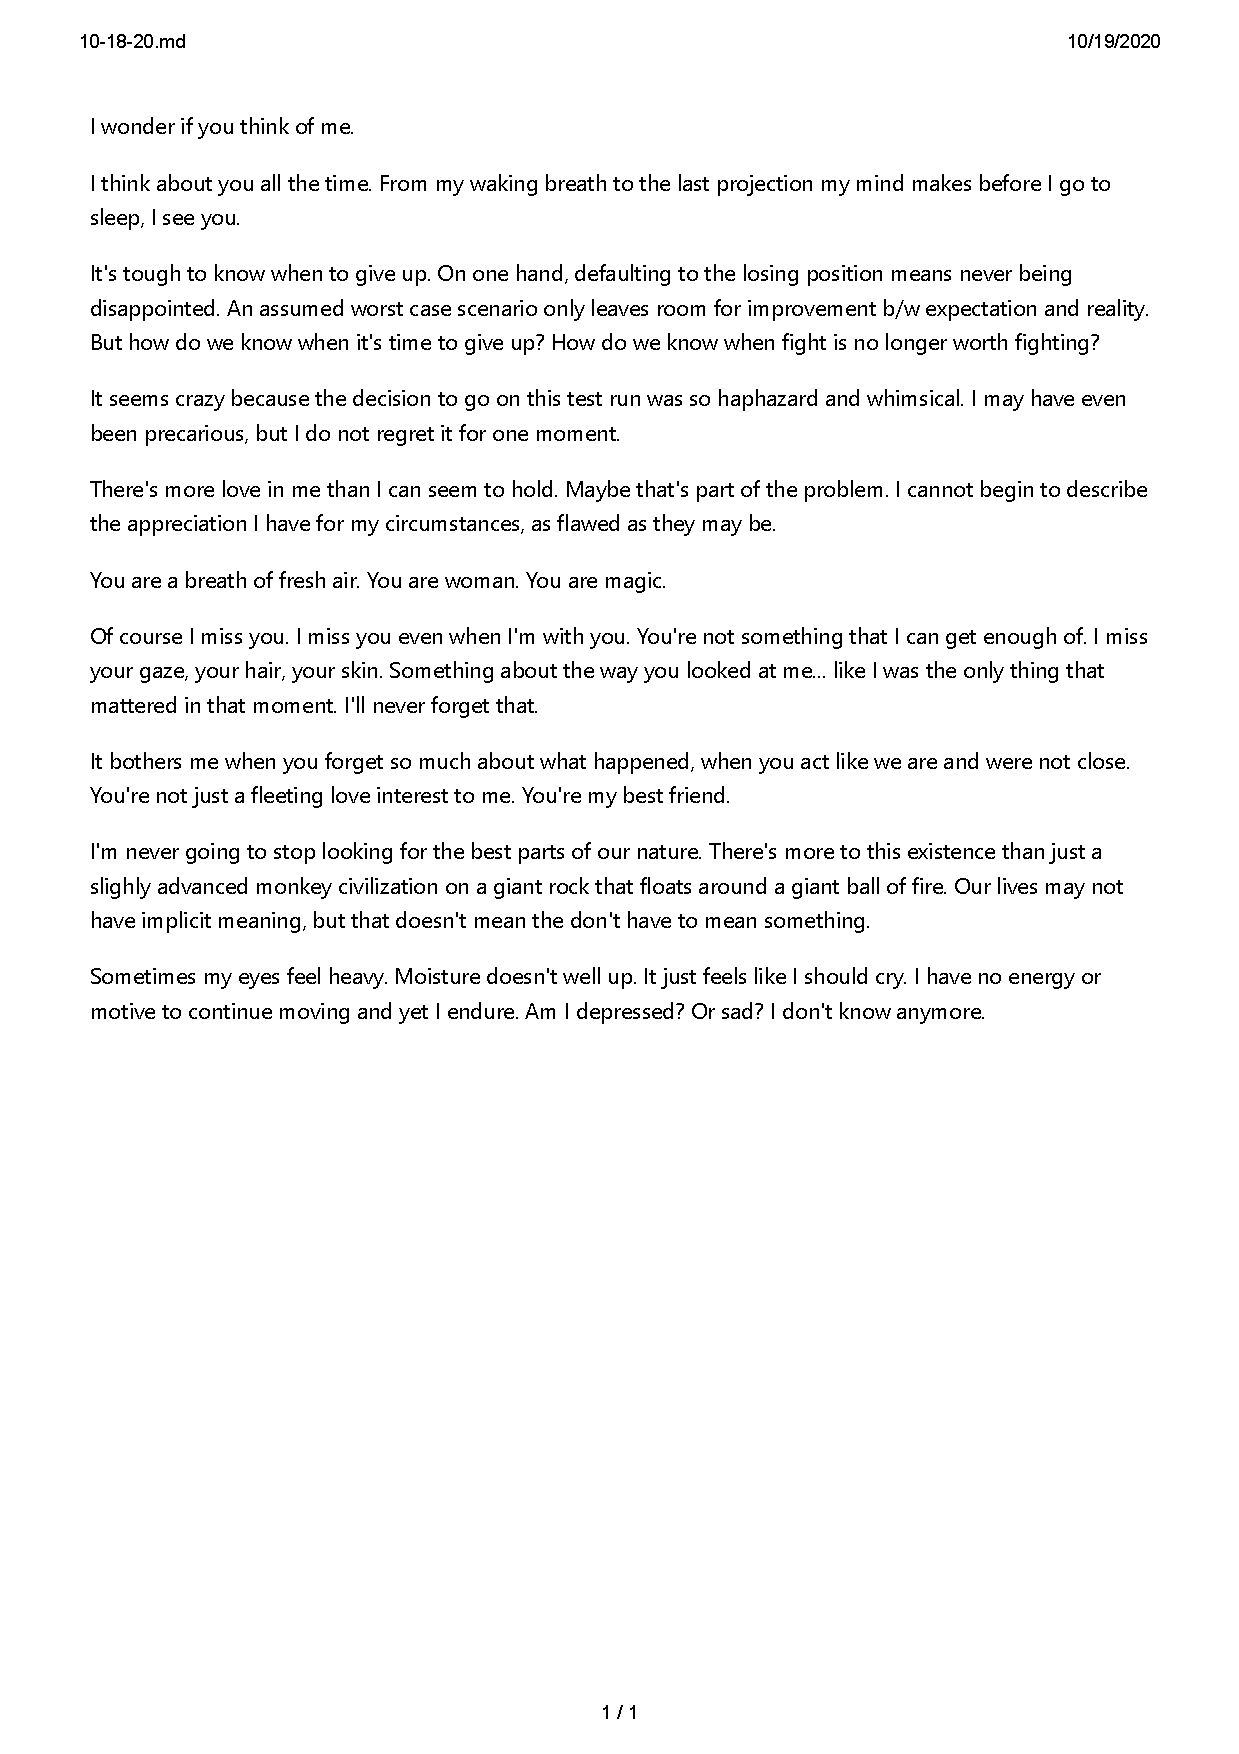
\includepdf[pages={1}]{subjects/entries/20-10-18.pdf}






% Bibliography
\bibliography{master_references}

%%%%%%%%%
\end{document}
%%%%%%%%%

% Template Recipes

%Bold Text:
%	\textbf{}

%Inline code:
%	\lstinline{code}

%Note environment:
%	\begin{note}
%
%	\end{note}

%Remark environment:
%	\begin{remark}
%	  On Overleaf, please use \hologo{XeLaTeX} to compile articles in Chinese and \hologo{pdfLaTeX} to compile articles in English.
%	\end{remark}

%Listing (code) environment.
%	\begin{lstlisting}
%	tlmgr update --self
%	tlmgr update --all
%	print("hello world")
%	\end{lstlisting}

%Assumption environment:
%	\begin{assumption}
%		assumptions
%	\end{assumption}
